\section{Introduction}
\label{sec:introduction}
%%%%%%%%%%%%% 我们干了啥事 %%%%%%%%%%%%
% 1.在 few-shot SPR 上对 generic/surgical FM 做了简单对比，发现 generic FM（DINOv3）潜力很大
% 2.选择DINOv3作为generic FM，然后针对性设计了video适配的策略
% 3.考虑临床部署挑战，提出了异构蒸馏策略
% 4.我们实验丰富，public和private数据集都验证few-shot优势明显，实时性部分也极大提升

% 总结三大卖点：generic FM 适配、few-shot即可高acc、计算效率实时性轻量化
%%%%%%%%%%%%%%%%%%%%%%%%%%%%%%%%%%%%%%%%%%%%%



%%% 这一段讲手术阶段识别的临床背景，以及大模型之前的技术发展 %%%
% 先讲手术阶段识别的任务定义
% 锚定临床价值：手术阶段识别是智能手术室的核心基础任务，精准、实时的手术阶段划分对术中智能导航、手术风险预警、标准化手术教学、术后技能复盘评估、手术机器人辅助执行具有不可替代的临床价值，是实现外科手术智能化、规范化的关键支撑。
% 然后讲手术阶段识别AI的技术发展 
% 1 传统方法：HMM等统计方法，依赖人工特征设计，泛化能力极差，无法适配复杂手术场景；
% 2 深度学习初期：2D/3D CNN方法，依靠大规模标注手术数据驱动，严重依赖海量精准标注样本，算力开销大、小样本场景失效；
% 3 - 主流前沿方法：Transformer架构方法，虽提升了长时序视频建模能力，但依旧存在数据依赖度高、模型参数量大、推理速度慢、跨术式泛化性差的问题，难以满足临床实时部署需求。
% 段落收尾点出核心矛盾：现有方法高度依赖大规模专属手术标注数据，训练成本高、隐私风险大，且轻量化与识别精度、小样本性能无法兼顾，极大限制了临床落地应用。
\IEEEPARstart{S}{urgical} phase recognition (SPR), aiming at identifying
frame-wise surgical intentions from a complete procedure video, is a
fundamental task for intelligent operating rooms. It underpins intraoperative decision
support~\cite{vermeulen2023ultra}, real-time anomaly detection~\cite{mithany2023advancements},
and postoperative skill assessment~\cite{cao2023intelligent}, this task has witnessed continuous
research into spatiotemporal modeling over the past years.
In the early days, statistical methods like hidden Markov models
(HMMs)~\cite{blum2008modeling, padoy2012statistical} modeled the temporal relations in surgical
workflows, but their reliance on hand-crafted features limited generalization.
Convolutional neural networks (CNNs)~\cite{krizhevsky2012imagenet} enabled automatic feature
extraction, and while vanilla 2D CNNs~\cite{primus2018frame} classify each frame independently,
hybrid architectures with sequential modelling~\cite{yengera2018less, zisimopoulos2018deepphase}
and 3D CNNs~\cite{czempiel2020tecno} were developed to capture temporal dynamics.
Most recently, Transformer architectures~\cite{yang2024surgformer} have redefined the
state-of-the-art by modelling long-range dependencies.
Despite these advances, increasingly complex architectures impose heavier annotation and parameter demands, and current methods still cannot well
balance recognition accuracy with model lightweighting and real-time efficiency, which remains a
key clinical bottleneck hindering their deployment.


%%% 这一段梳理相关FM的进展，并且引出并回答问题:FM怎么选 %%%
% 引入FM技术变革+原理铺垫：视觉基础模型的兴起打破了传统任务驱动的训练范式，依托海量通用数据预训练习得的普适视觉先验，模型具备强大迁移能力，可通过少量下游样本快速适配新任务，为手术阶段识别的few-shot场景提供了可行的技术路径。
% generic FM介绍一波
% 然后也要讲 surgical也有人在做FM
% 然后很自然引出一个科学问题：FM到底咋选
% 立刻解答：不做全面公平的 FM 基准，只在 few-shot SPR 上做个简单对比；发现通用 FM（DINOv3）即便几乎未见过手术数据，仍展现出很强的 few-shot 泛化潜力。
The emergence of visual foundation models (FMs) has broken the traditional
task-driven training paradigm.
Pre-trained on massive data, FMs acquire universal visual priors with
strong transferability, enabling rapid adaptation to novel downstream tasks with
only a handful of annotated samples.
For 2D images, a rich family of generic FMs has been
proposed, ranging from self-supervised learning schemes such as the DINOv3~\cite{simeoni2025dinov3} to image-text contrastive learning models such as CLIP~\cite{radford2021learning}.
Video FMs such as VideoMAEv2~\cite{wang2023videomae}, InternVideo2~\cite{wang2024internvideo2}, and V-JEPA2~\cite{assran2025v}
further extend this paradigm to the temporal dimension by pre-training on
large-scale video corpora.
In parallel, surgical FMs~\cite{wang2023foundation,wang2025improving,dermyer2025endodino,yuan2024hecvl, yuan2024procedure, yuan2025learning,hu2024ophclip} have also emerged, which collect diverse
surgical datasets and adopt pre-training recipes similar to those of
generic FMs.
These FMs thus represent a promising solution to the annotation burden that hampers existing SPR methods.




%%% 这一段引出并回答问题:FM选了DINOv3，然后怎么用 %%%
% 首先DINOv3是 image-based 模型，我们怎么设计video适配
% 然后是考虑临床部署的硬件限制，以及临床的实时性要求，我们怎么提出异构蒸馏
% 然后cue到我们取得的效果 teaser图
A simple comparison over representative FMs on few-shot SPR reveals the strong
potential of the generic FM DINOv3, which generalizes well to surgical videos
despite having seen almost no surgical data. We therefore select DINOv3 as our
backbone and devise a spatiotemporal adaptation tuning scheme that equips
DINOv3 with temporal modeling using only a handful of learnable parameters. Specifically, this scheme comprises a salient spatial token selection (SSTS) module and a keyframe-prior temporal fusion (KPTF) module, which reinforce the model's few-shot inductive bias and help it overcome the spatiotemporal redundancy of surgical videos.
However, the resulting model DINO-SPR is still bound to the
ViT backbone of DINOv3, which limits its deployment flexibility and real-time
efficiency.
We therefore propose DINO-SPR Lite, an architecture-agnostic distillation
strategy that compresses the teacher into a lightweight student of any backbone
family.
To this end, we introduce a cross-attention projection (CAP) that bridges the
representational gap between the ViT teacher and students of different
architectures.
We further design a spatiotemporally-guided distillation (STGD) that transfers
the teacher's spatial and temporal intermediate signals, which matter most in
the few-shot regime where logit-level supervision alone is too sparse to guide
the student.
Fig.~\ref{fig:tradeoff} summarizes the performance-efficiency
trade-off, where DINO-SPR Lite substantially surpasses prior methods in
inference efficiency and achieves real-time inference on CPU.


\begin{figure}[t]
\centerline{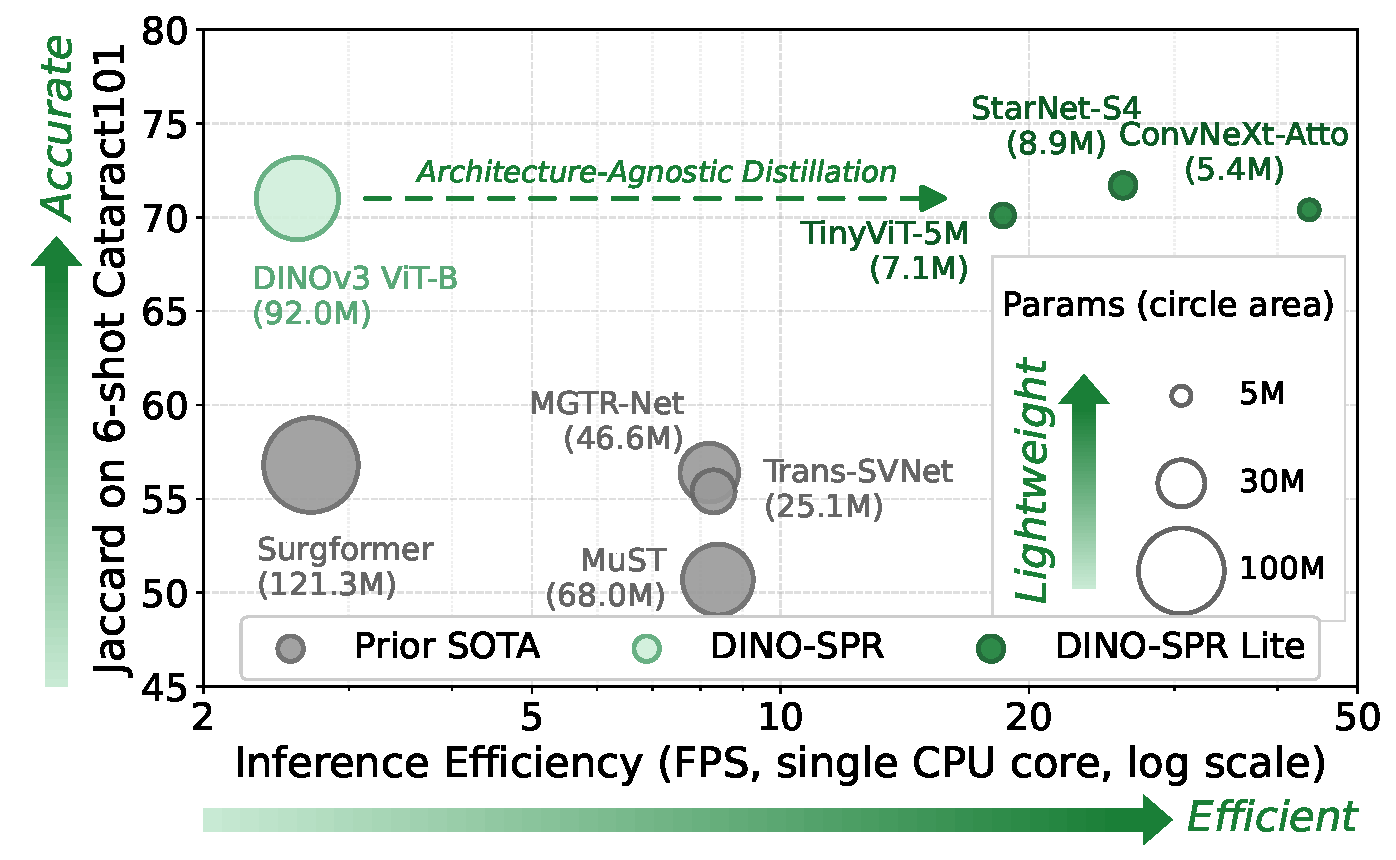
\includegraphics[width=\columnwidth]{resources/fig_computational_cost.pdf}}
\caption{6-shot Cataract101 Jaccard against inference efficiency on CPU, with circle area proportional to parameter count. Prior methods (gray) stay below 8.4\,FPS, while the DINO-SPR Lite students (dark green) match the DINO-SPR teacher (light green) at 18.6 to 43.7\,FPS.}
\label{fig:tradeoff}
\end{figure}


Our contributions could be summarized as follow:
% 贡献1：在 few-shot SPR 上对 representative 的 generic/surgical FM 做了简单对比，发现 generic FM DINOv3 的 few-shot 泛化潜力很大，由此选定 backbone
% 我们设计了video adaptation的策略，把image-based的DINOv3模型快速适配到surgical video任务
% 我们提出了异构模型蒸馏的方法，将few-shot适配后的DINOv3蒸馏到不同架构的轻量化模型，极大地提升了临床部署效率
% 5个手术阶段识别数据集，其中包含一个私有数据集，广泛验证了我们的算法，在few-shot场景下的准确率表现大幅超越previous SOTAs，并且在轻量化部署方面也明显更优
\begin{enumerate}
    \item We compare representative visual FMs on few-shot SPR and find that the
    generic DINOv3, although barely exposed to surgical data, already shows
    strong generalization, which motivates our choice of backbone.
    \item We devise a spatiotemporal adaptation tuning for DINOv3. The proposed SSTS and KPTF
    modules concentrate on the discriminative regions and key moments, enabling
    accurate adaptation under few-shot settings.
    \item We propose an architecture-agnostic distillation that compresses
    DINO-SPR into a lightweight student of any backbone, enabling flexible
    deployment above the 25\,FP on a single CPU with
    under 9M parameters.
    \item Extensive experiments on five SPR datasets,
    show that DINO-SPR substantially surpasses previous
    state-of-the-art under few-shot settings, while DINO-SPR Lite retains this
    performance with drastically fewer parameters and higher inference efficiency.
\end{enumerate}


